\chapter{概率}

连续从 $ (0,1) $ 区间随机取一个数(均匀分布), 直到所取的数之和超过1, 取出的数的个数为 $ N $, 求 $ N $ 的期望值.

解: 设第 $ i $ 次取出的数为 $ x_i $, 考虑 $ N\ge 2 $ 的概率, 只要满足 $ x_1<1 $, 这显然是恒成立的, 即 $ P(N\ge 2)=1 $.

考虑 $ N\ge 3 $ 的概率, 只要满足 $ x_1+x_2<1 $, 因为 $ x_i $ 为区间 $ (0,1) $ 上的均匀分布, 所以由几何概型知 $ P(N\ge 3) $ 的值是直线 $ x+y<1 $ 与两坐标轴围成的三角形的面积, $ P(N\ge 3)=\dfrac{1}{2} $.

类似的, $ P(N\ge 4)=P(x_1+x_2+x_3<1)=\dfrac{1}{6} $, 对应了平面 $ x+y+z<1 $ 和三个坐标轴围城的三棱锥的体积.

一般的, $ P(N\ge k+1) $ 的值为 $ k $ 维空间单位单纯形的体积, 为 $ \dfrac{1}{k!} $.

所求期望为
\begin{align*}
E(N) &= 1\cdot P(N=1) + 2\cdot P(N=2) + 3\cdot P(N=3) + \cdots \\
	&= 1(P(N\ge 1) - P(N\ge 2)) + 2(P(N\ge 2) - P(N\ge 3)) + \cdots \\
	&= P(N\ge 1) + P(N\ge 2) + P(N\ge 3) + \cdots \\
	&= 1 + 1 + \frac{1}{2!} + \frac{1}{3!} + \cdots \\
	&= e
\end{align*}


举一反三: 连续投掷飞镖, 飞镖落点为正方形范围内的均匀分布, 靶子最初是正方形的内切圆, 每次飞镖命中靶子后, 靶子直径会缩小至过命中点的最短弦长, 靶子中心仍不变. 例如下图. 直到飞镖没有命中靶子时游戏结束, 求投掷飞镖次数的期望.

\begin{wrapfigure}{o}{4.2cm}
\vspace{-1em}
\definecolor{wrwrwr}{rgb}{0.3803921568627451,0.3803921568627451,0.3803921568627451}
\definecolor{rvwvcq}{rgb}{0.08235294117647059,0.396078431372549,0.7529411764705882}
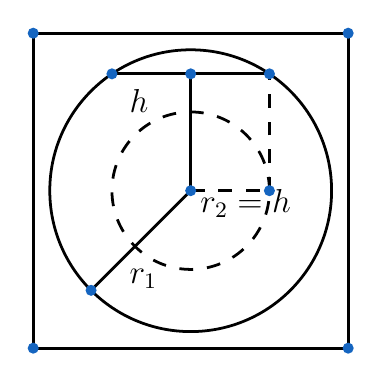
\begin{tikzpicture}[scale=2]
\coordinate (O) at (0,0);
\coordinate (A) at (-1,-1);
\coordinate (B) at (1,-1);
\coordinate (C) at (1,1);
\coordinate (D) at (-1,1);
\coordinate (X) at (0.5,0);

\coordinate (E) at (-0.5,0.741978595);
\coordinate (N) at (0,0.741978595);
\coordinate (F) at (0.5,0.741978595);

\coordinate (M) at (-0.6326658817810729,-0.632665881781073);
\tkzMarkRightAngle[line width=1pt,size=0.1](O,N,F);

\draw [line width=1pt] (A) -- (B) -- (C) -- (D) -- cycle;
\draw [line width=1pt] (O) circle (0.8947246704655265cm);
\draw [line width=1pt] (E)-- (F);
\draw [line width=1pt] (O)-- (M);
\draw [line width=1pt,dash pattern=on 5pt off 5pt] (X)-- (F);
\draw [line width=1pt] (O)-- (N);
\draw [line width=1pt,dash pattern=on 5pt off 5pt] (O) circle (0.5cm);
\draw [line width=1pt,dash pattern=on 5pt off 5pt] (O)-- (X);
\draw (0.0,0.06706007576871736) node[anchor=north west] {\large $r_2=h$};
\draw (-0.4503439003382287,-0.4339390629048399) node[anchor=north west] {\large $r_1$};
\draw (-0.4503439003382287,0.707046630673026) node[anchor=north west] {\large $h$};
\foreach \p in {A,B,C,D,E,F,M,N,O,X}
	\fill[fill=rvwvcq,thick] (\p) circle (1pt);

\end{tikzpicture}
\end{wrapfigure}
\mbox{}
解: 设靶心位于原点, 正方形区域边长为2. 不妨设第 $ i $ 次投掷靶子半径为 $ r_i $, 其中 $ r_1=1 $, 飞镖落在 $ (x_i,y_i) $ 处. 靶子半径收缩的条件为: $ (x_i^2+y_i^2) + r_{i+1}^2 = r_i^2 $, 可以推出
\begin{align*}
r_k^2 &= r_{k-1}^2 - (x_{k-1}^2 + y_{k-1}^2) \\ 
r_{k-1}^2 &= r_{k-2}^2 - (x_{k-2}^2 + y_{k-2}^2) \\ 
		& \vdots \\ 
	r_2^2	&= r_1^2 - (x_1^2+y_1^2)
\end{align*}

对上面的一系列等式求和, 可得
\[
r_k^2=r_1^2-\sum_{i=1}^{k-1}{(x_i^2+y_i^2)}.
\]

设游戏结束时投掷次数为 $ N $, 则 $ N \ge k $ 对应
\[
 r_1^2-\sum_{i=1}^{k-1}{(x_i^2+y_i^2)} > 0.
\]

$ k = 2 $ 时, 满足条件的状态集合为 $ (x_1^2+y_1^2) < 1 $, 即圆形内部, $ P(N\ge 2)=\dfrac{\pi}{4} $; 

$ k = 3 $ 时, 满足条件的状态集合为 $ (x_1^2+y_1^2+x_2^2+y_2^2) < 1 $, 即四维球体内部, 概率为四维球体与四维正方体的体积之比;

之后的 $ k $ 对应了6维, 8维等情况. 一般地, $ 2n $ 维球体体积公式为: $ V=\dfrac{\pi^n}{n!}R^{2n} $.

所以所求期望为
\begin{align*}
E(N)  &= 1\cdot P(N=1) + 2\cdot P(N=2) + 3\cdot P(N=3) + \cdots \\
	&= 1(P(N\ge 1) - P(N\ge 2)) + 2(P(N\ge 2) - P(N\ge 3)) + \cdots \\
	&= P(N\ge 1) + P(N\ge 2) + P(N\ge 3) + \cdots \\
	& = 1 + \frac{\pi}{4} + \frac{(\pi/4)^2}{2!} + \cdots \\
	& = \exp(\frac{\pi}{4})
\end{align*}


%------------------------------------------------------------------------------%
\newpage
\noindent 微分方程与连续采样均匀分布直到和超过1的问题.

连续从 $ (0,1) $ 区间随机取一个数 (均匀分布), 直到所取的数之和超过1, 取出的数之和为 $ S $, 求 $ S $ 的期望值.

解: 设第 $i$ 次取出的数为 $x_i$, 考虑更一般的问题: 直到所取的数之和超过 $t$ 结束, 取出的数之和的期望为 $f(t)$, 其中$t <= 1$. 记$\displaystyle A_k = \sum_{n=1}^k x_i$, 可见
\[ f(t) = E(A_N \ | A_{N-1} < t, A_N >= t) .\]

下面分情况讨论.

在 $x_1 > t$ 的情况下, 所取的数就是 $x_1$, 所取数之和的期望为 
\[E(x_1\ | x_1 > t) = \int_t^1{x}\ \mathrm{d}x = \frac{1-t^2}{2} ;\]

在 $x_1 < t$ 的情况下, 例如 $x_1 = u < t$, 则需要重复这个操作直到后面所取数之和超过 $t - u$, 于是所取数之和的期望为 
\[
E(A_N \ | x_1 < t, A_{N-1} < t, A_N >= t) = \int_0^t{u + f(t - u)}\ \mathrm{d}u = \frac{t^2}{2} + \int_0^t f(x)\ \mathrm{d}x .
\]

两部分合起来得:
\[f(t) = \frac{1-t^2}{2} + \frac{t^2}{2} + \int_0^t f(x)\ \mathrm{d}x = \frac{1}{2} + \int_0^t f(x)\ \mathrm{d}x .\]

将$t = 0$代入得 $f(0) = \dfrac{1}{2}$, 再两边求导得: $f'(t) = f(t) $, 可以解得 $f(t) = \dfrac{e^t}{2}$.

令 $t=1$, 得到 $S$ 的期望为 $\dfrac{e}{2}$.

~

连续从 $ (0,1) $ 区间随机取一个数 (均匀分布), 直到所取的数之和超过1, 取出的数个数为 $ N $, 求 $ N $ 的期望值.

解: 定义 $F(x)$ 为连续从 $ (0,1) $ 区间均匀取一个数, 直到所取的数之和超过 $x$, 所取出的数的个数的期望值, 这里 $x$ 限制在 $[0,1]$ 范围. 则要求的就是 $F(1)$. 

为了求一般的 $F(x)$ 的值, 考虑取出的第一个数, 分两种情况讨论: 

若第一个数大于 $x$, 概率为 $1-x$, 取数个数为 1.

若第一个数小于等于 $x$, 若取到 $t$, 概率为 $\mathrm{d}t$, 则取数个数期望为 $1 + F(x-t)$.

两种情况加起来, 得:
\begin{align*}
F(x) &= (1-x)\cdot 1 + \int_0^x{(1+F(x-t))}\ \mathrm{d}t \\
&= 1 + \int_0^x{F(x-t)}\ \mathrm{d}t \\
&= 1 + \int_x^0{-F(u)}\ \mathrm{d}u \\
&= 1 + \int_0^x{F(u)}\ \mathrm{d}u
\end{align*}
求导可得 $F'(x) = F(x)$, 并且初值为 $F(0) = 0$. 解得 $F(x) = e^x$. 于是 $F(0) = e$.


%------------------------------------------------------------------------------%
\newpage
\noindent 压垮骆驼的最后一根稻草的重量.

骆驼最大负重为 1, 有一堆稻草, 每一根重量都是 $(0,1)$ 上独立的均匀分布, 依次往骆驼身上放稻草, 直到超过最大负重, 求最后放上去的稻草重量的期望值.

解: 令第 $i$ 次放置的稻草重量为 $x_i$, 前 $n$ 次放置的稻草总重量为 $s_n = x_1+x_2+\cdots+x_n$. 定义函数 $g_n(x)$ 为取 $n$ 棵稻草的总重量小于 $x$ 的概率, 其中 $x\in(0,1)$. 那么由几何概型可知 $g_n(x)$ 就是 $x_1+x_2+\cdots+x_n < x$ 的概率, 它等于 $n$ 维单位等腰直角三角形的体积, 即
\[g_n(x) = \mathrm{Prob}(s_n < x) = \frac{x^n}{n!} .\]
再定义函数 $f_n(x)$ 为事件 $s_n < 1 < s_n + x$ 发生的概率, 即取了 $n$ 个稻草没有达到最大负重, 但再取一个重量为 $x$ 的稻草就会超重. 将事件拆成两个不等式, 再重新改写一下就是 $1-x < s_n < 1$, 可见有
\begin{align*}
f_n(x) &= \mathrm{Prob}(s_n<1) - \mathrm{Prob}(s_n<1-x) \\
&= g_n(1) - g_n(1-x) \\
&= \frac{1-(1-x)^n}{n!} .
\end{align*}
对所有的 $n$ 求和得到最后一根稻草重量为 $x$ 的概率为
\[f(x) = \sum_{n=0}^{\infty}{f_n(x)} = e - e^{1-x} .\]
于是最后一根稻草重量的期望值为:
\begin{align*}
E &= \int_0^1 x\cdot f(x)\ \mathrm{d}x \\
&= \int_0^1 x(e-e^{1-x})\ \mathrm{d}x \\
&= \frac{e}{2}x^2+(x+1)e^{1-x}\bigg|_0^1 \\
&= 2 - \frac{e}{2} \approx 0.6486.
\end{align*}

%------------------------------------------------------------------------------%
\newpage

\noindent 来自 Paul Nahin

一栋大楼有 $G,1,2,\cdots,N$ 层, 有一部电梯, 在各楼层均可以停留. 某人从 $G$ 层上电梯, 要去第 $M$ 层, 与他一起上电梯的还有另外 $K$ 个人, 他们去往各楼层的概率相同 ($G$层除外). 问某人到达第 $M$ 层之前, 电梯平均会停多少次.

~

解: 定义随机变量 $I_i$, 若电梯在第 $i$ 层停留, 则 $I_i = 1$, 否则 $I_i = 0$. 又设 $X$ 为到达第 $M$ 层之前电梯停留的次数之和, 则$\displaystyle X = \sum_{i=1}^{M-1}I_i$, $\displaystyle E(X) = \sum_{i=1}^{M-1} E(I_i)$, 而
\[E(I_i) = 0\times P(I_i = 0) + 1\times P(I_i=1) = P(I_i=1)\]
也就是说 $E(I_i)$ 等于电梯在第 $i$ 层停留的概率, 或 $K$ 个人中有人去第 $i$ 层的概率, 这里 $1\le i\le M - 1$. 可以根据全部 $K$ 个人都不去第 $i$ 层的概率来算, 也就是
\[
P(I_i=1) = 1 - (1-\frac{1}{N})^K
\]
于是
\[
E(X) = (M-1)\left(1-(1-\frac{1}{N})^K\right)
\]

~

\noindent 类似问题

有一个公平的 $N$ 面骰子, 独立地掷出 $K$ 次, 问掷出的不同点数的个数期望是多少.

解: 令 $X_i$ 表示 $K$ 次掷骰子是否至少出现一次 $i$ 点, 等于 1 表示出现过, 否则等于 0. 那么所求期望为:
\[E = E(X_1)+E(X_2)+\cdots+E(X_N) = N\cdot E(X_1) .\]
并且
\[
E(X_1) = 1\cdot\mathrm{Prob}(X_1=1)+0\cdot\mathrm{Prob}(X_1=0) = \mathrm{Prob}(X_1=1) = 1-(1-\frac{1}{N})^K ,
\]
所以最终期望为:
\[E = K\left(1-(1-\frac{1}{N})^K \right) .\]

%------------------------------------------------------------------------------%
\newpage
\noindent 来自 Paul Nahin (Ballot Theorem)

两人 $P$ 和 $Q$ 竞选某个职位, 最终的得票数分别为 $p$ 和 $q$, 且 $p>q$. 于是 $P$ 胜出. 在唱票过程中 $P$ 的得票数可能领先或落后于 $Q$, 取决于唱票时选票的排列顺序. 

求唱票过程中 $P$ 的票数自始至终都领先于 $Q$ 的概率.

~

解: 以横轴为唱票进度, 纵轴为 $P$ 累积领先的票数, 画出唱票结果.
\begin{figure*}[htbp]
\centering
\begin{tikzpicture}[scale=1]
\coordinate (O) at (0,0);
\coordinate (A) at (1,1);
\coordinate (AA) at (1,-1);
\coordinate (B) at (2,2);
\coordinate (BB) at (2,-2);
\coordinate (C) at (3,1);
\coordinate (CC) at (3,-1);
\coordinate (D) at (4,2);
\coordinate (DD) at (4,-2);
\coordinate (E) at (5,3);
\coordinate (EE) at (5,-3);
\coordinate (F) at (6,2);
\coordinate (FF) at (6,-2);
\coordinate (G) at (7,1);
\coordinate (GG) at (7,-1);
\coordinate (H) at (8,0);
\coordinate (I) at (9,-1);
\coordinate (J) at (10,0);
\coordinate (K) at (11,1);
\draw[->,line width=1pt] (-1,0) -- (12,0) node[right] {$x$};
\draw[->,line width=1pt] (0,-4) -- (0,4) node[above] {$y$};
\draw[line width=1pt,red] (O)--(A)--(B)--(C)--(D)--(E)--(F)--(G)--(H);
\draw[line width=1pt] (H)--(I)--(J)--(K);
\draw[line width=1pt,blue,dashed] (O)--(AA)--(BB)--(CC)--(DD)--(EE)--(FF)--(GG)--(H);
\foreach \p in {O,A,B,C,D,E,F,G,H,I,J,K,AA,BB,CC,DD,EE,FF,GG}
	\fill[fill=black,draw=black,thick] (\p) circle (1.25pt);
\end{tikzpicture}
\end{figure*}

每次$x$ 增加1, $y$要么增加1, 要么减少1. $P$ 一直领先于 $Q$ 意味着从原点出发后, 折线图一直在 $x$ 轴上方, 也不会与 $x$ 轴相交. 不管唱票顺序如何, 最终 $P$ 净领先的票数是固定的. 即不管折线图怎么拐, 终点的位置都是固定的. 如果折线某时刻到达了 $x$ 轴上或 $x$ 轴下方, 后面必然会经过 $x$ 轴重新回到上方.

考虑唱票序列的第一张票, 若是投给 $Q$ 的, 则此时已经不能满足 $P$ 一直领先于 $Q$ 的条件, 发生的概率为$\dfrac{q}{p+q}$. 若第一张是投给 $P$ 的, 后面仍然可能出现票数持平或者被 $Q$ 反超的情况. 找到第一次持平的时刻, 并将此前的投票结果依次取反, 将得到一个新的序列. 例如上图的序列$\color{red}{PPQPPQQQ}\color{black}{QPP}$, 以 $P$ 开头, 但是中间落后于 $Q$. 构造的新序列为 $\color{blue}{QQPQQPPP}\color{black}{QPP}$, 两个序列的最终得票结果是一样的, 但新序列总是以 $Q$ 开头. 

任意一个以 $P$ 开头的并中途达到过平手状态的序列都与一个以 $Q$ 开头的序列一一对应. 满足条件 A: $P$ 不是一直领先于 $Q$ 的序列数量是满足条件 B: 第一张票是 $Q$ 的序列数量的两倍. 因此 $P$ 一直领先于 $Q$ 的概率为:
\[1 - \frac{2q}{p+q} = \frac{p-q}{p+q} .\]


%------------------------------------------------------------------------------%
\newpage 

\noindent 来自 Paul Nahin 

有一个圆形的葡萄干布丁, 上面有 $n$ 个葡萄干, 它们在布丁上的位置的独立的均匀分布. 求离圆心最远的葡萄干到圆心距离的期望值.

~

解: 设布丁的半径为 $R$, 葡萄干到圆心的距离为随机变量 $x_i$, 则$x_i$的 pdf 为
\[p(x_i=r) = \frac{2\pi r\cdot\mathrm{d}r}{\pi R^2} = \frac{2r\cdot\mathrm{d}r}{R^2}.\]
则 $\max\{x_i\}$ 的 cdf 为:
\[p(\max\{x_i\} \le x) = \left( \int_0^x{\frac{2r}{R^2} \mathrm{d}r}\right)^n = \left(\frac{x}{R}\right)^{2n}\]
对应的 pdf 为: 
\[p(\max\{x_i\} = r) = \frac{2n\cdot r^{2n-1}}{R^{2n}} .\]
期望值为:
\[\int_0^R{\frac{2n\cdot r^{2n-1}}{R^{2n}}\cdot r}\ \mathrm{d}r = \frac{2n}{2n+1}\cdot \frac{r^{2n+1}}{R^{2n}}\bigg|_0^R = \frac{2n}{2n+1}\cdot R\]



%------------------------------------------------------------------------------%
\newpage

\noindent 来自 Paul Nahin

有 $n$ 个独立同分布的随机变量 $X_1, X_2, \cdots, X_n$, 都是 $(0,1)$ 上的均匀分布, 求他们中的最大值除以最小值的商大于 $k$ 的概率, 其中 $k \ge 1$.

~

解: 令 $U = \min\{X_i\}, V = \max\{X_i\}$, 先计算 $U,V$ 的联合分布的累计密度函数 
$$F_{U,V}(u,v) = \mathrm{Prob}(U\le u, V\le v) ,$$ 
再计算联合分布的概率密度函数 
$$f_{U,V}(u,v) = \frac{\partial^2}{\partial u\partial v}F_{U,V}(u,v). $$

分两部分计算 $F_{U,V}(u,v)$. 当 $u\ge v$ 时, 条件A: $\min\{x_i\}\le u$ 被条件B: $\max\{x_i\}\le v$所包含了, 所以 
$$F_{U,V}(u,v) = \mathrm{Prob}(U\le u, V\le v) = \mathrm{Prob}(V\le v) = v^N,\ \ u\ge v , $$ 
表达式与$u$无关, 从而
$$f_{U,V}(u,v) = 0,\ \ u\ge v .$$

另一方面, 当 $u < v$ 时, $U\le u$ 且 $V\le v$ 意味着所有 $X_i \le v$, 且至少有一个 $X_i \le u$. 只要计算所有 $X_i \le v$的概率, 并减去所有 $X_i$ 都在 $(u,v)$ 范围内的概率, 于是:
\begin{align*}
F_{U,V}(u,v) &= \mathrm{Prob}(U\le u, V\le v) \\
&= \mathrm{Prob}(V\le v) - \mathrm{Prob}(u\le X_1,X_2\cdots,X_N\le v) \\
&= v^N - (v-u)^N,\ \ u < v.\\
f_{U,V}(u,v) &= N(N-1)(v-u)^{N-2}, \ \ u < v.
\end{align*}

要求的事件为最大值除以最小值的商大于 $k$, 即 $V > kU$, 全部位于 $u<v$ 一侧, 所以所求概率为:
\[
\mathrm{Prob}(V > kU) = \int_0^1\int_0^{v/k}{N(N-1)(v-u)^{N-2}}\ \mathrm{d}u\mathrm{d}v
\]

~

注: 可以求出$V$的 CDF 为:
\begin{align*}
F_V(v) &= \mathrm{Prob}(\max\{X_i\} \le v)\\
&= \mathrm{Prob}(X_1\le v, X_2\le v, \cdots, X_n\le v) \\
&= v^N .
\end{align*}

类似的求出 $U$ 的CDF 为:
\begin{align*}
F_U(u) &= \mathrm{Prob}(\min\{X_i\} \le u) = 1- \mathrm{Prob}(\min\{X_i\} > u)\\
 &= 1 - \mathrm{Prob}(X_1 > u, X_2 > u, \cdots, X_n > u)\\ 
 &= 1 - (1-u)^N.
\end{align*}

进而可以计算 $U,V$ 的 PDF:
\begin{align*}
f_U(u) &= \frac{\mathrm{d}}{\mathrm{d}u}F_U(u) = N(1-u)^{N-1} \\
f_V(v) &= \frac{\mathrm{d}}{\mathrm{d}v}F_V(v) = Nv^{N-1} .
\end{align*}

但是 $U,V$ 不独立, 所以$f_{U,V}(u,v) \neq f_U(u)\cdot f_V(v)$.


%------------------------------------------------------------------------------%
\newpage
一根木棍上独立地取两个随机点, 将木棍分成三段, 每个随机点都是均匀分布. 求三段可以构成三角形的概率.

~

\noindent 直接解法: 

设木棍长度为1, 能构成三角形当且仅当分成的三段长度都小于$\dfrac{1}{2}$. 木棍两个端点记作 $A,B$. 下面计算存在长度超过 $\dfrac{1}{2}$ 的一段的概率.
\begin{figure*}[htbp]
\centering
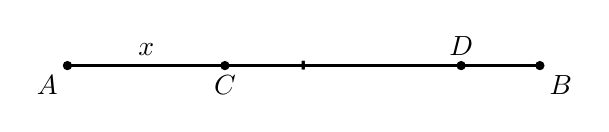
\begin{tikzpicture}[]
\coordinate[label=below left:$A$] (A) at (0,0);
\coordinate[label=below right:$B$] (B) at (6,0);
\coordinate[label=below:$C$] (C) at (2,0);
\coordinate[label=above:$D$] (D) at (5,0);
\draw [line width=1pt] (A) -- (B) node [midway,sloped] {$\bracevert$};
\draw[] (1,0) node[anchor=south] {$x$};
\foreach \p in {A,B,C,D}
	\fill[fill=black,draw=black,thick] (\p) circle (1.25pt);
\end{tikzpicture}
\end{figure*}

考虑所选两个随机点 $C,D$ 的位置, 设 $AC$ 的长度为 $x$. 当 $x\in[0,\dfrac{1}{2})$ 时, 如果 $D$ 落在 $AC$ 上, 则 $CB$ 一定是超过 $\dfrac{1}{2}$ 的, 概率为 $x$, 且其他段不会超过 $\dfrac{1}{2}$; 如果 $D$ 落在 $CB$ 上, 则可能是 $CD$ 或者 $DB$ 长度超过 $\dfrac{1}{2}$, 概率都是 $\dfrac{1}{2} - x$. 三种情况合起来概率为 $1 - x$. 对 $x$ 积分, 得
\[\int_0^{\frac{1}{2}}{(1-x)}\ \mathrm{d}x = \frac{3}{8}.\]
而当 $x\in[\dfrac{1}{2},1]$ 时, 是对称的情况, 存在一段长度超过 $\dfrac{1}{2}$ 的概率也是 $\dfrac{3}{8}$. 所以三段不能构成三角形的概率为 $\dfrac{3}{4}$, 可以构成三角形的概率为 $\dfrac{1}{4}$.

~

\noindent 图形解法

考虑一个高为 1 的等边三角形 $ABC$, 三角形内一点 $P$ 到各边的距离分别为 $x,y,z$, 则 $x + y + z = 1$, 如下图.
\begin{figure*}[htbp]
\centering
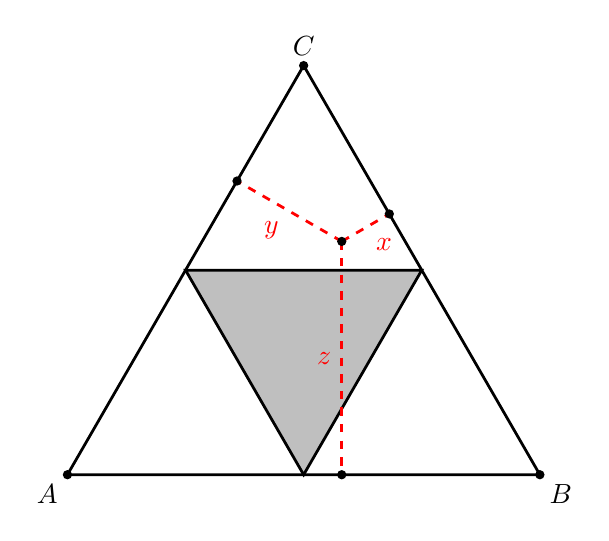
\begin{tikzpicture}[]
\coordinate[label=below left:$A$] (A) at (-3,0);
\coordinate[label=below right:$B$] (B) at (3,0);
\coordinate[label=above:$C$] (C) at (0,5.196);
\coordinate[] (D) at (0,0);
\coordinate[] (E) at (-1.5,2.598);
\coordinate[] (F) at (1.5,2.598);
\coordinate[] (P) at (0.484,2.963);
\coordinate[] (G) at (0.484,0);
\coordinate[] (H) at (-0.846,3.73);
\coordinate[] (I) at (1.088,3.312);
\draw [line width=1pt] (A) -- (B) -- (C) -- cycle;
\fill[gray!50] (D) -- (E) -- (F) -- cycle;
\draw [line width=1pt] (D) -- (E) -- (F) -- cycle;
\draw [dashed,red,line width=1pt] (P) to[edge label'=$z$] (G);
\draw [dashed,red,line width=1pt] (P) to[edge label=$y$] (H);
\draw [dashed,red,line width=1pt] (P) to[edge label'=$x$] (I);
\foreach \p in {A,B,C,G,H,I,P}
	\fill[fill=black,draw=black,thick] (\p) circle (1.25pt);
\end{tikzpicture}
\end{figure*}

每个 $P$ 的位置对应了一个将木棍分成三段的方式. 而只有当 $P$ 落在中间小三角形内部时, 才满足 $x,y,z$ 都小于 $\dfrac{1}{2}$, 所以能构成三角形的概率为小三角形与大三角形面积之比, 等于 $\dfrac{1}{4}$.

%------------------------------------------------------------------------------%
\newpage
\noindent By Mr.Why

不超过 90 的正整数中随机选出 5 个不同的数, 求选出的数中最大数的期望.

~

\noindent 直接解法:

若最大数为 $N$, 则它对结果的贡献为:
\[\frac{N\cdot C_{N-1}^4}{C_{90}^5}=\frac{N}{C_{90}^5}\cdot\frac{(N-1)!}{4!(N-5)!}=\frac{5}{C_{90}^5}\cdot\frac{N!}{5!(N-5)!}=\frac{5}{C_{90}^5}\cdot C_{N}^{5}\]
所求期望为:
\[E = \frac{5}{C_{90}^5}\cdot\sum_{N=1}^{90}{C_N^5}\]
对于这个求和, 由 $C_m^m=C_{m+1}^{m+1}$ 和 $C_n^m + C_n^{m-1}=C_{n+1}^m$, 可得:
\begin{align*}
C_m^m + C_{m+1}^m+\cdots+C_n^m &= C_{m+1}^{m+1}+ C_{m+1}^m + C_{m+2}^m + \cdots + C_n^m \\
&= C_{m+2}^{m+1} + C_{m+2}^m + \cdots + C_n^m \\
&= \cdots \\
&= C_{n+1}^{m+1}.
\end{align*}
所以 
\[E=\frac{5}{C_{90}^5}\cdot C_{91}^6 = \frac{455}{6}.\]

~

\noindent 图形解法

\begin{wrapfigure}{o}{5cm}
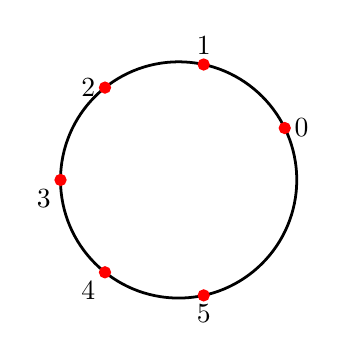
\begin{tikzpicture}[cap=round,scale=1.5]
\tikzstyle{axes}=[line width=1pt]
\coordinate[label=right:$0$] (A) at (0.8982934325496409,0.43939607308006734);
\coordinate[] (G) at (0.8982934325496409,-0.43939607308006734);
\coordinate[label=above:$1$] (B) at (0.21206921921340208,0.9772546476032836);
\coordinate[label=below:$5$] (F) at (0.21206921921340208,-0.9772546476032836);
\coordinate[label=left:$2$] (C) at (-0.6234898077068194,0.7818314778043369);
\coordinate[label=below left :$4$] (E) at (-0.6234898077068194,-0.7818314778043369);
\coordinate[label=below left:$3$] (D) at (-1,0);
\coordinate (X) at (1,0);
\coordinate[] (O) at (0,0);
\draw [line width=1pt] (O) circle (1cm);
\foreach \p in {A,B,C,D,E,F}
	\fill[fill=red,draw=red,thick] (\p) circle (1.2pt);
\end{tikzpicture}
\end{wrapfigure}

考虑一个圆的内接正 91 边形, 在其上随机选出 6 个顶点, 再选择一个作为 0 号点, 按逆时针方向其他5个点分别是 1 到 5 号. 于是从 0 号到其他号沿逆时针方向经过的边数就对应从不超过 90 的正整数中随机选出 5 个不同数的一个选法, 最大的数就是 0 号到 5 号点需要经过的边数, 它也是总边数减去 5 号点逆时针到 0 号点需要经过的边数. 

一旦初始的 6 个顶点选定, 它们将圆周分成了 6 段弧, 它们的地位是对称的, 因为 0 号点在这 6 个点中的位置是随机的, 意味着每段弧都有相同的概率成为 5 号点到 0 号点的那一段. 于是这一段的平均长度是圆周长的 $1/6$, 所以0号点到5号点的长度期望就是 $91\times(1-1/6) = 455/6$ .


%------------------------------------------------------------------------------%
\newpage
\noindent 反败为胜的概率

$A,B$ 两支队伍水平相当, 已知其中一支队伍在上半场落后, 且上下半场净比分不相同(因而最终没有平局). 求最终它反败为胜的概率是多少. 假设上半场和下半场的表现是独立的.

~

解: 在任意半场比赛中, $A$ 净胜 $B$ 任意分数的概率等于 $B$ 净胜 $A$ 同样分数的概率. 假设一支队伍半场净胜另一支队伍 $x$ 分和 $y$ 分的概率分别是 $p$ 和 $q$, 不失一般性, 可以设 $x > y$, 则考虑上下半场$A$ 净胜 $B$ 的分数, 下面事件发生的概率相等:
\begin{figure*}[htbp]
\centering
\begin{tabular}{c|c|c}
\hline
上半场 & 下半场 & 是否反败为胜 \\ \hline
$+x$ & $+y$ & No \\ \hline
$+y$ & $+x$ & No \\ \hline
$+x$ & $-y$ & No \\ \hline
$+y$ & $-x$ & Yes \\ \hline
$-x$ & $+y$ & No \\ \hline
$-y$ & $+x$ & Yes \\ \hline
$-x$ & $-y$ & No \\ \hline
$-y$ & $-x$ & No \\ \hline
\end{tabular}
\end{figure*}

无论 $x,y$ 是多少, 反败为胜的情况占比都是相同的. 因此总体而言, 上半场落后的队伍在下半场反超的概率为 $\dfrac{1}{4}$.

注: 如果去掉上下半场净比分不相同的限制, 则有可能 $x=y$, 此时不会出现反败为胜的情况, 需要更多条件才能进一步计算.


%------------------------------------------------------------------------------%
\newpage

国际象棋的马随机游走, 平均多少步回到原来的位置.
\begin{figure*}[htbp]
\centering
\begin{tikzpicture}[line cap=round,line join=round,>=triangle 45,x=1cm,y=1cm]
\clip(-1.,-0.1) rectangle (5,4.1);
\draw [help lines,line width=2pt,color=black] (0,0) grid (4,4);
\draw (0.5,3.5) node[anchor=center] {$A$};
\draw (1.5,3.5) node[anchor=center] {$B$};
\draw (2.5,3.5) node[anchor=center] {$C$};
\draw (3.5,3.5) node[anchor=center] {$D$};
\draw (0.5,2.5) node[anchor=center] {$E$};
\draw (1.5,2.5) node[anchor=center] {$F$};
\draw (2.5,2.5) node[anchor=center] {$G$};
\draw (3.5,2.5) node[anchor=center] {$H$};
\draw (0.5,1.5) node[anchor=center] {$I$};
\draw (1.5,1.5) node[anchor=center] {$J$};
\draw (2.5,1.5) node[anchor=center] {$K$};
\draw (3.5,1.5) node[anchor=center] {$L$};
\draw (0.5,0.5) node[anchor=center] {$M$};
\draw (1.5,0.5) node[anchor=center] {$N$};
\draw (2.5,0.5) node[anchor=center] {$O$};
\draw (3.5,0.5) node[anchor=center] {$P$};
\end{tikzpicture}
\end{figure*}

考虑小规模的情形. 在 $ 4\times 4 $ 的棋盘内, 马在任意一个格子都可以经过有限步到达其他所有的格子. 

假设初始在 $ A $ 点, 分别以 $ 1/2 $ 的概率到达 $ G $ 和 $ J $ 两点, 假设从这两点回到 $ A $ 点的期望步数为 $ E_A(G) $ 和 $ E_A(J) $, 则所求值为 
\[ E_A = \frac{1}{2}[E_A(G) + 1] + \frac{1}{2}[E_A(J)+1] = 1 + \frac{1}{2}[E_A(G)+E_A(J)]. \]

进一步, 从 $ G $ 出发可以到达 $ A, I, N, P $ 四个点, 于是
\[ E_A(G)= 1+\frac{1}{4}[ E_A(A) + E_A(I) + E_A(N) + E_A(P) ]. \]

然后又可以推出其他点的关系, 得到一个 16 元方程组, 并注意到 $ E_A(A)=0 $, 可以解出 $ E_A(A),\cdots,E_A(P) $, 进而求出期望次数.

~

另一种思路是根据马尔科夫过程达到稳态时的状况. 一种快速求出稳态的方法如下. 

考虑马从每个格子 $ x $ 进行一步跳跃可能到达的邻居状态个数 $ Adj(x) $. 比如 $ A $ 能到达 2 个, $ B $ 能到达 3 个, $ F $ 能到达 4 个. 每个格子放 $ Adj(x) $ 个马, 这样一次跳跃后, 每个格子的所有马都跳到其中一个邻居状态, 而邻居状态也各有一个马跳到这个格子补充, 这样整个棋盘马的分布没变, 也就是稳态. 于是稳态下在每个点 $ x $ 停留的时间比例是 $ p(x) = Adj(x)/\sum{Adj(i)} $.  

\begin{wrapfigure}{o}{3cm}
\vspace{-1em}
\begin{tikzpicture}[->,>=stealth',shorten >=1pt,auto,node distance=2cm,semithick]
\tikzstyle{every state}=[]
\node[state] (A) {$x$};
\node[state] (B) [right of=A] {$\bar{x}$};
\path (A) edge  [bend left] node [above] {r} (B)
(A) edge [loop above] node {$1-r$} ()
(B) edge [loop above] node {$1-q$} ()
(B) edge  [bend left] node [below] {$q$} (A);
\end{tikzpicture}
\end{wrapfigure}
\mbox{}
现在只关注一个特定状态 $ x $, 可以将原来的马尔科夫过程简化成两个状态, 其中稳态以 $ p(x) $ 的概率位于 $ x $ 而以 $ 1 - p(x) $ 的概率位于 $ x $ 以外的点, 用 $ \bar{x} $ 表示. $ x $ 将以概率 $ r $ 转移到 $ \bar{x} $, 而 $ \bar{x} $ 将以概率 $ q $ 转移到 $ x $. 由稳态概率可得 $ p(x) r = (1-p(x))q $, 于是 
\[ q = \frac{p(x)r}{1-p(x)}. \]

在这个简化版的马尔科夫过程里, 可知从 $ \bar{x} $ 状态到达 $ x $ 的平均时间为 
\[ E_x(\bar{x}) = q\cdot 1 + (1-q)\cdot (1+E_x(\bar{x})). \]
解得 $ E_x(\bar{x}) = \dfrac{1}{q}.$ 所以两次到达 $ x $ 之间的时间平均为 
\[ (1-r)\cdot 1 + r\cdot (1+E_x(\bar{x})) = 1 + r\cdot E_x(\bar{x}) = 1 + \frac{r}{q} = \dfrac{1}{p(x)} .\]

本问题中 $ r = 1 $, 但结果其实和 $ r $ 无关, 所以这个结论也适用于一般的马尔科夫过程: 已知稳态下到达给定状态的概率是 $ p $, 则两次到达这个状态平均需要的转移次数为 $ 1/p $.

%------------------------------------------------------------------------------%
\newpage

袋子中有 $ 10 $ 个红球, $ 20 $ 个蓝球, $ 30 $ 个绿球, 随机将这些球一个一个取出, 问红球最先被取完的概率.

考虑最后一个球是什么颜色, 如果是蓝色, 概率是 $ 1/3 $, 再考虑的剩下 $ 40 $ 个球中, 最后一个是绿色的概率, 为 $ 3/4 $; 如果所有的最后一个颜色是绿色, 概率为 $ 1/2 $, 剩下 $ 30 $ 个球最后一个是蓝色的概率是 $ 2/3 $. 所以这两种情况加起来得到红球最先被取完的概率: 
\[ p = \frac{1}{3} \times \frac{3}{4} + \frac{1}{2} \times \frac{2}{3} = \frac{7}{12} .\]

%------------------------------------------------------------------------------%
\newpage
\noindent 来自网络: 

音乐播放器里存了 100 首歌, 编号 1 到 100, 按顺序排列. 播放器有两个按键: Next 和 Random. 如果当前播放的是第 $i$ 号, 按 Next 就会跳到下一首, 也就是第 $i+1$ 号, 如果是 100 号的话就会跳到 1 号. 如果按下 Random 键, 就会随机等可能地跳转到 100 首歌地任意一首, 当然也可能还是刚刚播放的那一首. 某人最偏爱编号 42 的那首歌. 播放器启动时是随机的一首, 他想通过尽可能少的按键次数调整到他最爱的歌, 问他的最佳策略是什么, 所需按键次数的期望值是多少?

~

\noindent 解:

令 $x$ 表示当前状态下需要按多少次 Next 能到达 42 号. 则 $ 0\le x\le 99$. 在最优策略下, 不会出现按了 Next 后又按 Random 的操作, 因为任何时候按 Random, 之后期望的按键次数都是一样的, 不必先按一次 Next 再按 Random. 所以最优策略一定是先按 0 次或多次 Random 键, 直到足够接近 42 号, 然后一直按 Next 键到达目标.

假设临界距离为 $k$, 当 $x\le k$时, 就按 Next, 否则就按 Random. 设 $N$ 为随机状态下的期望按键次数, $E(x)$ 为状态为 $x$ 时期望的按键次数, 则:
\[E(0) = 0, E(1) = 1, \cdots, E(k) = k,\]
\[E(k+1) = E(k+2) = \cdots = E(99) = 1 + N .\]

另一方面, 因为 $\displaystyle N = \frac{1}{100}\sum_{n=0}^{99}{E(n)}$, 代入可得
\[ N = \frac{k}{2} + \frac{100}{k+1} - 1, \]
因为 $k$ 是非负整数, 当 $k=13$ 时, $N=\dfrac{177}{14}$ 达到最小.

%------------------------------------------------------------------------------%
\newpage

圆周上随机选三个点, 求构成的三角形包含圆心的概率.
\begin{figure*}[htbp]
\centering
\definecolor{rvwvcq}{rgb}{0.08235294117647059,0.396078431372549,0.7529411764705882}
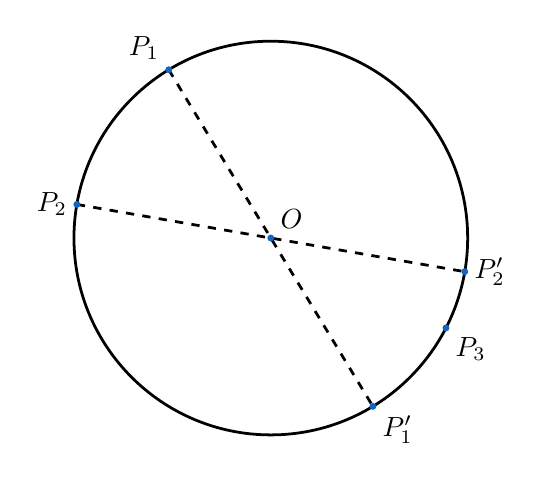
\begin{tikzpicture}[scale=0.5]
\def\xa{2.5928244165910157}
\def\ya{4.2751914044554145}
\def\xb{4.926495524400919}
\def\yb{0.854190756246933}
\coordinate[label=above left:$P_1$] (P1) at (-\xa,\ya);
\coordinate[label=below right:$P_1'$] (P11) at (\xa,-\ya);
\coordinate[label=left:$P_2$] (P2) at (-\xb,\yb);
\coordinate[label=right:$P_2'$] (P22) at (\xb,-\yb);
\coordinate[label=below right:$P_3$] (P3) at (4.448267345577948,-2.28318146941169);
\coordinate[label=above right:$O$] (O) at (0,0);

\draw [line width=1pt] (O) circle (5cm);
\draw [line width=1pt,dash pattern=on 3pt off 3pt] (P2)-- (P22);
\draw [line width=1pt,dash pattern=on 3pt off 3pt] (P1)-- (P11);
\foreach \p in {P1,P11,P2,P22,P3,O}
	\fill[fill=rvwvcq,thick] (\p) circle (2.5pt);

\end{tikzpicture}
\end{figure*}

固定 $ P_1 $, 假设 $ P_2 $ 与 $ P_1 $ 夹角是 $ \theta \in [0,\pi] $, 只有当 $ P_3 $ 位于 $ P_1P_2 $ 对侧的弧 $ P_1'P_2' $ 上时, 三角形才能包含圆心. $ P_3 $ 符合条件的概率为 $ \dfrac{\theta}{2\pi} $, 而 $ P_2 $ 与 $ P_1 $ 夹角是 $ \theta $ 的概率恒为 $ \dfrac{1}{\pi} $, 积分可得:
\[ \int_0^\pi{ \frac{1}{\pi}\cdot \frac{\theta}{2\pi} \text{d}\theta} =\frac{1}{4} \]

\noindent 另一个思路:

任选 $ P_1, P_2, P_3 $, 并考虑它们关于圆心的镜像 $ P_1', P_2', P_3' $, 在 $ P_1 $ 和 $ P_1' $ 中选一个, $ P_2 $ 和 $ P_2' $ 中选一个, $ P_3 $ 和 $ P_3' $ 中选一个, 一共有 8 种可能, 其中有且只有两种情况能构成包含圆心的三角形. $ P_i $ 和 $ P_i' $ 的地位是对等的, 所以概率是 $ \dfrac{1}{4} $.

或者固定 $ P_3 $, 任取 $ P_1, P_2 $, 并考虑它们的镜像 $ P_1', P_2' $, 类似上面的想法, 4 种可能的三角形里, 有且仅有一种包含圆心. 每一个包含圆心的三角形都对应 3 个等可能的不包含圆心的三角形, 所以概率也是 $ \dfrac{1}{4} $.

~

\noindent 推广问题: 球面上随机取四个点, 构成的四面体包含球心的概率是多少. (答案是 $ \dfrac{1}{8} $.)

~

\noindent 类似的问题: 圆形的池塘里有 $n$ 只鸭子, 求它们都位于同一个半圆内的概率.

假设有 $n$ 个位置 $P_1, P_2, \cdots, P_n$, 并考虑它们关于圆心的镜像 $P_1', P_2', \cdots, P_n'$. 每一对互为镜像的点选一个放鸭子, 共选出$n$个位置, 这样共有 $2^n$ 种取法, 显然这 $2^n$ 种取法都是对称的. 

那么哪些取法可以让 $n$ 个鸭子在同一个半圆内呢? 注意到互为镜像的两个位置不可能出现在同一个半圆内(不考虑边界情况, 或者半圆范围规定为左开右闭的区间), 沿着任一直径将圆分成两半, 每个半圆内总是包含 $n$ 个点, 并且编号恰好都是 $1,2,\cdots,n$, 比如$\{P_1, P_2', P_3',\cdots,P_n\}$, 另一个半圆包含这些点的镜像. 所以每个直径都对应了两个满足要求的取法. 而位于辐角值相邻的两个位置之间的各条直径对应的是相同的划分, 所有直径会产生 $n$ 种本质上不同的划分. 于是共有 $2n$ 种取法可以让 $n$ 个鸭子在同一个半圆内.

最后, 所有鸭子位于同一个半圆内的概率是 $p=\dfrac{2n}{2^n} = \dfrac{n}{2^{n-1}}$.

当 $n=3$ 时, 三个点位于同一半圆等价于三点构成的三角形不包含圆心, 概率为 $\dfrac{3}{4}$, 也是能对上的.


%------------------------------------------------------------------------------%
\newpage

单位圆内随机取两个点, 求它们的距离的期望.

~

最直接的解法是遍历两个点的位置, 并求一个四重积分. 比较困难.

不妨假设所求的期望是 $L$, 如果我们考虑一个稍大一点的圆, 在半径为 $(1+\Delta r)$ 的圆内随机取两个点, 它们的距离期望值就是 $(1+\Delta r)L$. 其中 $\Delta r$ 是无穷小量. 这个稍大的圆由两部分组成, 其一是原来的单位圆, 其二是单位圆外宽度为 $\Delta r$ 的圆环. 
在大圆内随机取两个点, 可能有 $3$ 种情况: 
\begin{enumerate}
\item 两个点都落在单位圆内;
\item 两个点都落在圆环上;
\item 各有一个点在单位圆内和圆环上.
\end{enumerate}
下面分别讨论每个情况的概率$p_1, p_2, p_3$和对应的距离期望 $L_1, L_2, L_3$.

情况1. 概率为单位圆与大圆面积之比的平方, 期望就是原问题的期望
\begin{align*} 
p_1 &= \left( \frac{1}{(1+\Delta r)^2} \right)^2 = \frac{1}{(1+\Delta r)^4},\\
L_1 &= L.
\end{align*} 

情况2. 概率为圆环与大圆面积之比的平方.
\[p_2 = \left( \frac{(1+\Delta r)^2 - 1}{(1+\Delta r)^2} \right)^2 .\]
这里偷个懒, 可以不计算 $L_2$. 只要知道它小于大圆的直径, 即 $L_2 < 2(1+\Delta r)$.

情况3. 概率为 $ p_3 = 1 - p_1 - p_2 $. 

\begin{figure*}[htbp]
\centering
\definecolor{ududff}{rgb}{0.30196078431372547,0.30196078431372547,1}
\definecolor{uuuuuu}{rgb}{0.26666666666666666,0.26666666666666666,0.26666666666666666}
\begin{tikzpicture}[scale=2]
\tikzstyle{axes}=[line width=1pt]
\clip(-1.5,-1.45) rectangle (1.6,1.6);
\draw [line width=1pt] (0,0) circle (1cm);
\draw (0.75,0.92) node[anchor=north] {$\Delta r$};
\draw (0.85,-0.05) node[anchor=north] {$2$};
\draw (0.0,-0.1) node[anchor=north] {$1$};
\draw [line width=1pt] (0,0) circle (1.2cm);
\draw [line width=1pt] (-1,0)-- (0.4,0.5);
\begin{scope}[style=axes]
    \draw[->] (-1.4,0) -- (1.4,0) node[right] {$x$};
    \draw[->] (-1,-1.4) -- (-1,1.4) node[above] {$y$};
\end{scope}
\begin{scriptsize}
\draw [fill=uuuuuu] (0,0) circle (1pt);
\draw [fill=uuuuuu] (1,0) circle (1pt);
\draw [fill=ududff] (-1,0) circle (1pt);
\draw [fill=ududff] (0.4,0.5) circle (1pt);
\end{scriptsize}
\end{tikzpicture}
\end{figure*}
\noindent 若圆环内的点落在内径上, 因为对称性, 可以按上图建立坐标系, 单位圆的圆心在 $(1,0)$, 写成极坐标的形式为 $r = 2\cos\theta $, 其中 $-\pi/2 < \theta < \pi/2$.
距离的期望值为:
\[ L_3'= \frac{1}{\pi}\int_{-\frac{\pi}{2}}^{\frac{\pi}{2}}\int_0^{2\cos\theta} r\cdot r\mathrm{d}r \mathrm{d}\theta = \frac{32}{9\pi},\]
这里的双重积分前面除以 $\pi$ 是因为均匀分布下取到圆内每个点的概率密度都是 $1/\pi$. 

类似地, 若圆环内的点落在外径上, 仍然固定外径上的点在原点上. 大圆的极坐标形式为 $ r = 2(1+\Delta r)\cos\theta$, 距离期望值为:
\[ L_3'' = \frac{1}{\pi(1+\Delta r)^2}\int_{-\frac{\pi}{2}}^{\frac{\pi}{2}}\int_0^{2(1+\Delta r)\cos\theta} r\cdot r\mathrm{d}r \mathrm{d}\theta = \frac{32}{9\pi}(1+\Delta r).\]

实际上, 圆环内采样点不会正好落在内径或外径上, 因此期望距离应该介于二者之间: $ L_3' < L_3 < L_3''$.

综合三种情况, 并且令 $\Delta r \rightarrow 0$, 用 $o(\Delta r)$ 表示 $\Delta r$ 的高阶无穷小.
\begin{align*}
p_1 &= \frac{1}{(1+\Delta r)^4} = \left(1-\frac{\Delta r}{1+\Delta r}\right)^4 = 1 - 4\Delta r + o(\Delta r) \\
p_2 &= \left( \frac{(1+\Delta r)^2 - 1}{(1+\Delta r)^2} \right)^2 = o(\Delta r) \\
p_3 &= 1 - p_1 - p_2 = 4\Delta r + o(\Delta r)
\end{align*}

根据前面的分析, 有 
\begin{align*}
(1+\Delta r)L &= p_1L_1 + p_2L_2 + p_3L_3 \\
&= (1-4\Delta r)L+ 4\Delta r\cdot\frac{32}{9\pi} + o(\Delta r) \\
5\Delta r\cdot L &= \frac{128}{9\pi}\Delta r + o(\Delta r) \\
L &= \frac{128}{45\pi}.
\end{align*}

~

\noindent 补充说明:

假设单位圆内两个随机点到圆心的距离分别是 $r_1$ 和 $r_2$, 若它们的较大者等于 $r$ ,由前面情况 3 的结论可知, 两点间距离的期望为 $\dfrac{32}{9\pi}r$. 

然后考虑条件 $\mathrm{max}(r_1,r_2)=r$ 的概率密度, 为了求pdf, 可以先求cdf: 
\[ P(\mathrm{max}(r_1,r_2) < r) = P(r_1<r)\cdot P(r_2<r) = \left( \frac{\pi r^2}{\pi} \right)^2 = r^4.\]
对应的 pdf为 $P(\mathrm{max}(r_1,r_2) = r) = 4r^3$. 于是, 对所有条件进行积分得到期望:
\[
L = \int_0^1 \frac{32}{9\pi}r\cdot 4r^3 \mathrm{d}r = \frac{128}{45\pi}.
\]

%------------------------------------------------------------------------------%
\newpage

\noindent Ross-Littlewood 悖论 (来源: A first course in probability, Sheldon Ross. 第 8 版.)

有一个无限容量的罐子和无限个球, 编号分别为 $ 1, 2, \cdots $. 先用了半天时间将第 1 至 10 号放进罐子, 并取出第 1 号球, 再用 $ 1/4 $ 天将第 11 至第 20 号球放进罐子, 并取出第 2 号球. 以后每次用前一次一半的时间放进 10 个球, 并取出罐子里编号最小的球. 这样一天结束时, 经过无限次操作后, 罐子里有多少球?

任意一个编号为 $ k $ 的球, 都会在第 $ k $ 次放球后被取出来, 所以罐子里不会有任何球.

但是, 如果换一种取法, 每次放完之后取出罐子里编号最大的球, 第一次放球后取出第 10 号, 第二次取出第 20 号, 等等, 每次都净增加 9 个球, 且不会被取出, 经过无限次操作后, 罐子里有无限个球.

如果每次放入球之后随机取出一个已有的球, 对于第 1 号球来说, 每次都不被取出的概率为 
\[ P_1 = \frac{9}{10}\cdot\frac{18}{19}\cdot\frac{27}{28}\cdots .\]
下面说明 $ P_1 $ 等于 0, 或乘积
\[ \frac{1}{P_1} = \frac{10\cdot 19\cdot 28\cdots}{9\cdot 18\cdot 27\cdots} = \prod_{k=1}^\infty{\frac{9k+1}{9k}} =\infty.\]

注意到
\begin{align*}
 \prod_{k=1}^\infty{\frac{9k+1}{9k}} &= \prod_{k=1}^\infty{\left(1+\frac{1}{9k}\right)} \\
	& > \prod_{k=1}^m{\left(1+\frac{1}{9k}\right)} \\
	&= \left(1+\frac{1}{9}\right)\left(1+\frac{1}{18}\right)\cdots\left(1+\frac{1}{9m}\right) \\
	& > \frac{1}{9} + \frac{1}{18} + \cdots + \frac{1}{9m} \\
	& = \frac{1}{9} \sum_{i=1}^m {\frac{1}{i}}
\end{align*}

当 $ m $ 趋于无穷时, 右边级数发散, 所以乘积是无穷大, 说明第 1 号球被留下的概率是 0. 其他球也是类似, 只不过和 1 号球留下的概率相比会相差一个常数倍, 但其实也是 0.

%------------------------------------------------------------------------------%
\newpage

空间中有一个边长为 $ 1 $ 的正方体, 位于 $xy$ 平面上方, 有一个沿 $z$ 轴的平行光, 照射到立方体后会在 $xy$ 平面上投下阴影, 立方体可以自由旋转, 求阴影面积的期望值.

\noindent 解: 

先考虑单个面的情况, 假设一个边长为 $1$ 的正方形的法线与 $z$ 轴夹角为 $\theta$, 那么它在 $xy$ 平面的投影面积为 $|\cos\theta|$. 而法线朝向为 $\theta$ 的概率密度为$\theta$对应的球面小圆环与整个球面的面积之比:$\dfrac{2\pi\sin\theta\Delta\theta}{4\pi}=\dfrac{1}{2}\sin\theta\Delta\theta$. 当法线遍历了所有方向的时候, 投影面积的平均值为:
\begin{align*}
 S_1 &= \int_0^\pi {\frac{1}{2}\sin\theta\cdot |\cos\theta|\ \mathrm{d}\theta} \\
&= \frac{1}{2}\int_0^{\pi/2} {\sin 2\theta \ \mathrm{d}\theta} \\
&= \frac{1}{2}.
\end{align*}

当平行光从正面进入立方体的其中一个面时, 必然会从另一个面的反面出去, 再打到 $xy$ 平面上, 于是, 每个面对阴影面积的贡献都有两次. 考虑立方体所有六个面合在一起投影面积就是 $3/2$.

需要补充一点, 假设以立方体的顶面朝向视为立方体的朝向, 顶面朝向北极的时候, 四个侧面朝向赤道. 
当顶面的法线朝向遍历整个球面时, 侧面的法线朝向的概率分布不一定和顶面一样.
例如, 不管顶面朝向什么方向, 我们总是可以绕顶面法线旋转立方体, 使得立方体的特定的一个侧面法线方向总是在 $z^+$ 半球.
因此需要对立方体朝向做更准确的定义. 除了考虑顶面法线朝向, 还要考虑顶面绕法线旋转的角度, 即 roll 角. 事实上, 更合理的定义立方体朝向的方式是按三维旋转群 $SO(3)$ 来定义. 当立方体的顶面在 $SO(3)$ 上均匀分布时, 其他所有的面也是 $SO(3)$ 上的均匀分布.

~

\noindent 延伸思考

先不着急求上面的积分式. 注意到平面上的任意多边形放在空间中并在 $xy$ 平面投影, 不难发现本质上和正方形的情况没有区别. 再考虑任意凸多面体, 光线从一个面进入必然会从另一个面离开, 所有面的对投影恰好贡献了两次. 假设多面体的表面积为 $S$, 那么平均的投影面积应该为 $\bar{S}=\dfrac{1}{2}{c}{S}$. 这里的$c$是待定系数, 且与多面体的形状无关. 事实上, $c$ 就是上面的积分式的值.

令凸多面体逐步逼近到球形, 此时不管朝向什么角度, 投影面积都是恒定的, $\bar{S} = \pi r^2$, $S=4\pi r^2$, 所以立刻得到 $c=\dfrac{1}{2}$. 回到原问题, 立方体的平均投影面积就是 $3/2$.


%------------------------------------------------------------------------------%
\newpage

设 $X_1, X_2, \cdots, X_n$ 是$(0,1)$ 上的均匀分布, 且两两之间独立, 求它们最大值和最小值之差的期望.

解: 直接根据定义求

\begin{align*}
\int_{[0,1]^n} {\max_{1\le i,j\le N}|x_i-x_j| \mathrm{d}V} &= n!\int_{1\ge x_n > x_{n-1}>\cdots >x_1\ge 0} {\max_{1\le i,j\le n}|x_i-x_j|} \mathrm{d}V\\
&= n!\int_0^1 \int_0^{x_n} \cdots \int_0^{x_2}{(x_n-x_1)}\ \mathrm{d}x_1\cdots\mathrm{d}x_{n-1}\mathrm{d}x_n\\
&= n!\int_0^1 \int_0^{x_n} \cdots \int_0^{x_3}{\left(x_n\cdot x_2-\frac{x_2^2}{2}\right)}\ \mathrm{d}x_2\cdots\mathrm{d}x_{n-1}\mathrm{d}x_n\\
&= n!\int_0^1 \int_0^{x_n} \cdots \int_0^{x_4}{\left(x_n\cdot\frac{x_3^2}{2}-\frac{x_3^3}{3!}\right)}\ \mathrm{d}x_3\cdots\mathrm{d}x_{n-1}\mathrm{d}x_n\\
&=\cdots\\
&=n!\int_0^1 \int_0^{x_n} {\left(x_n\cdot\frac{x_{n-1}^{n-2}}{(n-2)!}-\frac{x_{n-1}^{n-1}}{(n-1)!}\right)}\  \mathrm{d}x_{n-1}\mathrm{d}x_n\\
&=n!\int_0^1{\left(\frac{x_n^n}{(n-1)!} - \frac{x_n^n}{n!}\right)}\ \mathrm{d}x_n\\
&=(n-1)\int_0^1{x_n^n}\ \mathrm{d}x_n\\
&=\frac{n-1}{n+1}
\end{align*}

注意第一行是因为 $x_1,x_2,\cdots,x_n$ 的大小顺序关系有 $n!$ 种可能(不考虑相等), 这些情况都是对称的, 所以只需要考虑其中一种特定的顺序即可.















